\documentclass{ltjsarticle}
\usepackage{listings}
\lstset{%
 language={C},
 basicstyle={\small},%
 identifierstyle={\small},%
 commentstyle={\small\itshape},%
 keywordstyle={\small\bfseries},%
 ndkeywordstyle={\small},%
 stringstyle={\small\ttfamily},
 frame={tb},
 breaklines=true,
 columns=[l]{fullflexible},%
 numbers=left,%
 xrightmargin=0,%
 xleftmargin=3,%
 numberstyle={\scriptsize},%
 stepnumber=1,
 numbersep=1,%
 lineskip=-0.5%
}
\usepackage{graphicx}
\usepackage{amsmath}
\usepackage{mathtools}
\usepackage{url}
\mathtoolsset{showonlyrefs=true}
\title{}
\author{62304644 片山さくら}
\begin{document}
\maketitle

\section{設計方針・プログラム}


\subsection{実行環境}
\begin{list}{\labelitemi}{\leftmargin=1em}
  \item OS: Windows 11
  \item 開発環境: Visual Studio 2019 v142
  \item ビルドツール: MSbuild 16.11.2.50704
  \item コンパイラ: MSVC 19.29.30157 for x86
  \item C言語標準: C17
\end{list}

\subsection{使用ライブラリ}
\begin{list}{\labelitemi}{\leftmargin=1em}
  \item freeglut,glfw.3.4.0,glm.1.0.1 : グラフィック用(NuGetパッケージを使用)
\end{list}

\subsection{プログラムの動作}

プログラム全体の機能は、順列の生成、相異なる二分探索木の生成、二分探索木の高さの平均・分散の算出、二分木の描画である。
このプログラムはユーザーと標準入力やウィンドウを通して対話しながら動作する。

\subsection{プログラム中で使用する構造体の説明}

Node構造体に自身のキー、左右の子ノードへのポインタを持たせることで二分探索木を実装した。
binary\_tree.cに定義される関数を用いてNodeオブジェクトを生成、二分探索木として構成する事ができる。
また、Nodeオブジェクトのグラフィクス的な側面としてNodeGraphic構造体を定義した。NodeGraphicオブジェクトは
文字の色やエッジの色を保持し、tree\_graphic.cに定義される関数を用いて、構成済みの二分探索木を描画することができる。
NodeオブジェクトはNodeGraphicオブジェクトに依存せず生成や木の構成が可能である一方、NodeGraphicオブジェクトはNodeオブジェクトを
もとに生成される。

\subsection{プログラムの構成・概要}

ファイル構成

\begin{list}{\labelitemi}{\leftmargin=1em}
\item main.c : メイン関数
\item binary\_tree.c : 二分探索木の生成・ノードの追加削除・探索などの関数などを定義
\item tree\_analysis.c : 二分探索木の集合に対し、高さの平均・分散を算出する関数などを定義
\item tree\_graphic.c : 二分木の描画関数を定義
\item simulation\_graphic.c : 描画ループの実装
\item utility.c : 順列生成や階乗計算などの補助関数を定義
\item position.c : 座標を扱いやするするための関数を実装
\item list.c : 簡易的なリストの実装
\end{list}

\begin{list}{\labelitemi}{\leftmargin=1em}
\item binary\_tree.h : 二分探索木の構造体定義や関数のプロトタイプ宣言・Node構造体の定義
\item tree\_analysis.h : 二分探索木の集合に対する分析関数のプロトタイプ宣言
\item tree\_graphic.h : 二分木の描画関数のプロトタイプ宣言・NodeGrahic構造体の定義
\item simulation\_graphic.h : 描画ループのプロトタイプ宣言
\item utility.h : 補助関数のプロトタイプ宣言
\item position.h : 座標を扱うための関数のプロトタイプ宣言・XYi構造体の定義
\item list.h : 簡易的なリストのプロトタイプ宣言・List構造体の定義
\end{list}

\section{➀与えられた整数nまで自然数で構成される順列の生成}

\lstinputlisting[caption=utility.c]{../utility.c}

utility.cにおいて重要な関数は以下のとおりである。

\begin{list}{\labelitemi}{\leftmargin=1em}
\item calculate\_permutation : 与えられた整数nまでの順列のうちseedで始まる順列を全てlistに格納する関数
\item permutation\_num : 与えられた順列に対応する番号を返す関数
\item set\_permutation\_list : listに対し整数nまでの順列を全て格納する関数
\end{list}

set\_permutation\_list関数がcalculate\_permutation関数を呼び出すことで、与えられた整数nまでの順列を全てlistに格納する。
permutation\_num関数はcalculate\_permutation関数内で順列を格納するインデックスを算出するのに使われている。
permutation\_num関数により 1,2,3,4は0へ、4,3,2,1は23へと変換される。permutation\_test関数を実行することにより動作確認可能。

\textrm{permutation\_testの実行例}

\begin{align}
1 2 3 4\\
1 2 4 3\\
1 3 2 4\\
1 3 4 2\\
1 4 2 3\\
1 4 3 2\\
2 1 3 4\\
2 1 4 3\\
2 3 1 4\\
2 3 4 1\\
2 4 1 3\\
2 4 3 1\\
3 1 2 4\\
3 1 4 2\\
3 2 1 4\\
3 2 4 1\\
3 4 1 2\\
3 4 2 1\\
4 1 2 3\\
4 1 3 2\\
4 2 1 3\\
4 2 3 1\\
4 3 1 2\\
4 3 2 1\\
\end{align}

\section{➁ 生成した順列の順に数を入力したときに生成される相異なる二分探索木の列挙}

\lstinputlisting[caption=binary\_tree.c]{../binary\_tree.c}

binary\_tree.cにおいて重要な関数は以下のとおりである。

\begin{list}{\labelitemi}{\leftmargin=1em}
\item get\_key\_record : あるノードを根とした部分木を前順に探索しキーの値を配列に格納する関数
\item get\_different\_trees : 整数nまでの順列を順に二分探索木に入力し、生成したすべての相異なる二分探索木の根へのポインタをリストに格納する関数
\end{list}

とある順列を二分探索木に入力する際、同様の配置を取る二分探索木が生成することがある。
そのため構造的な重複を避けるために、二分木の構造とノードを前順で探索し順に記録して出来た順列が
一対一に対応することを利用し、get\_different\_trees関数内ではutility.cのpermutation\_num関数を用いて二分木にIDを付け
重複したものは記録しないようにしている。


\textrm{実行例 n=4の場合 (なお、完全二分木の場合文字は赤、AVL木の場合文字は青、それ以外は黒で表示される。)}

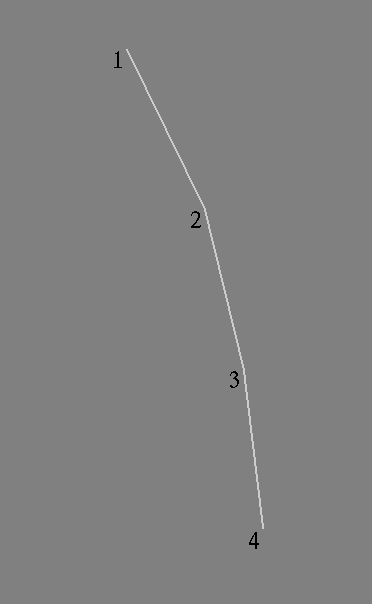
\includegraphics[width=4cm]{2.png}
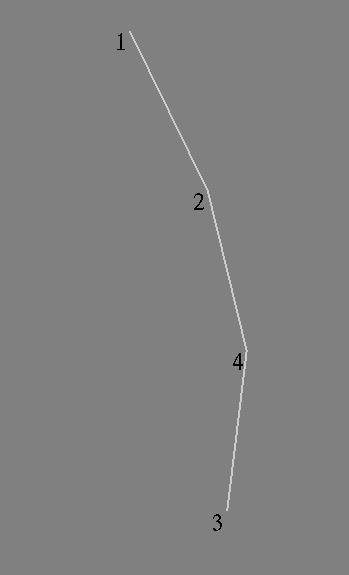
\includegraphics[width=4cm]{3.png}
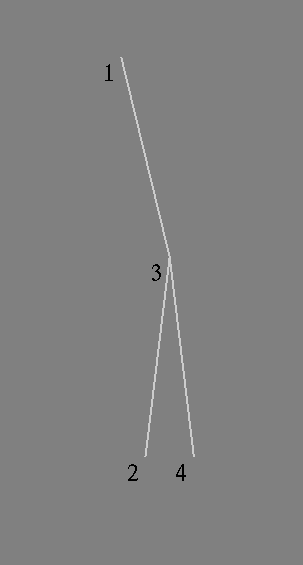
\includegraphics[width=4cm]{4.png}
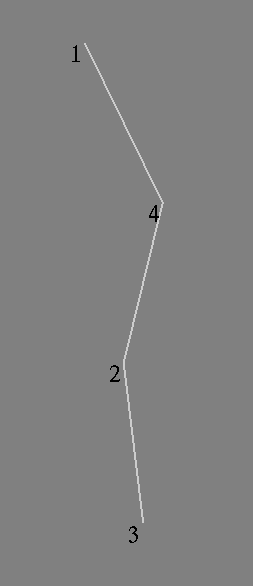
\includegraphics[width=4cm]{5.png}
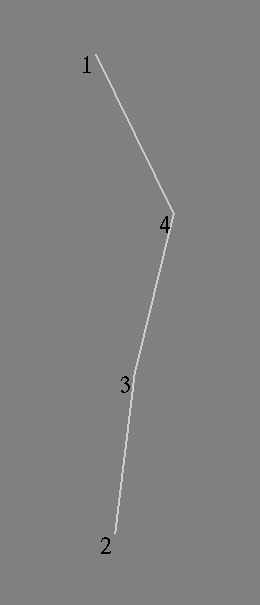
\includegraphics[width=4cm]{6.png}
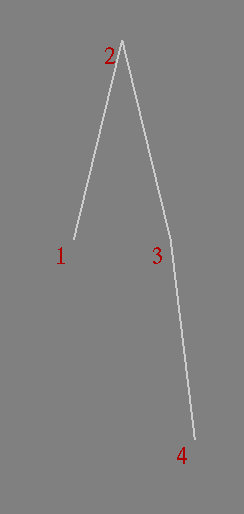
\includegraphics[width=4cm]{7.png}
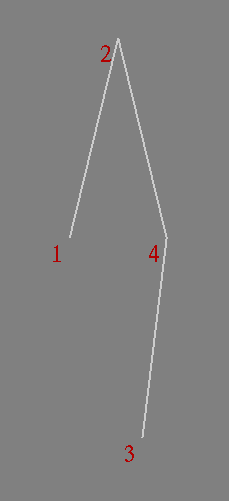
\includegraphics[width=4cm]{8.png}
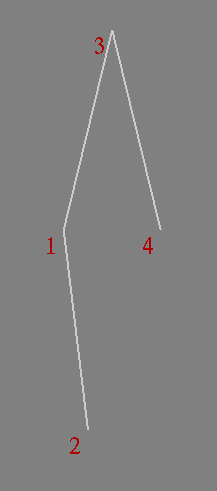
\includegraphics[width=4cm]{9.png}
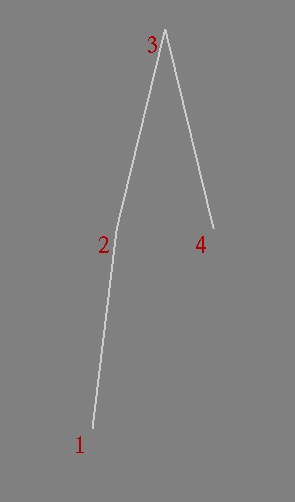
\includegraphics[width=4cm]{10.png}
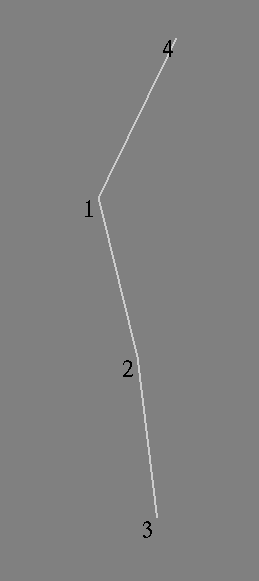
\includegraphics[width=4cm]{11.png}
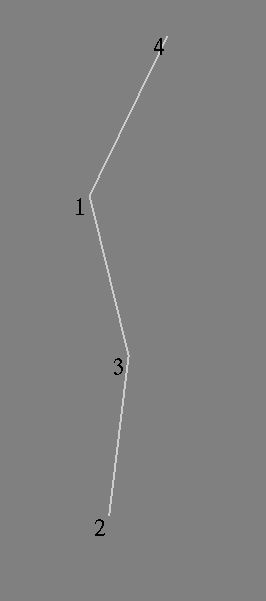
\includegraphics[width=4cm]{12.png}
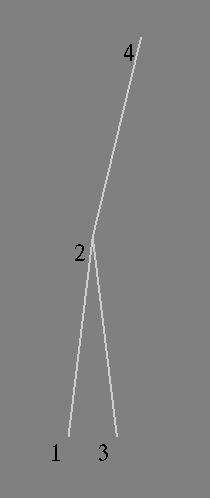
\includegraphics[width=4cm]{13.png}
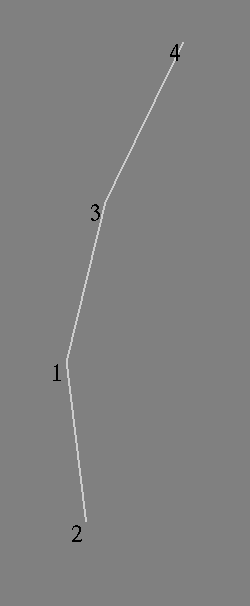
\includegraphics[width=4cm]{14.png}
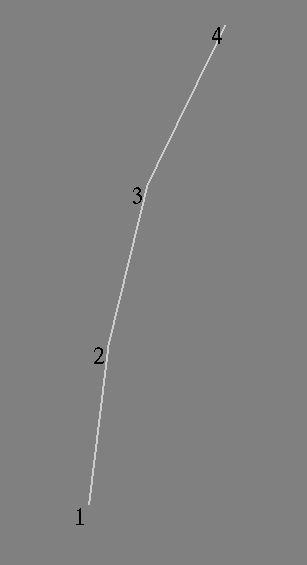
\includegraphics[width=4cm]{15.png}

上の結果はSQ7の結果と一致する。

nが1から9までの場合についてそれぞれの木の高さの平均と分散を算出した。

\begin{center}
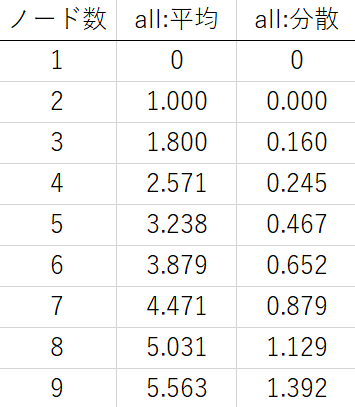
\includegraphics[width=5cm]{all_t.png}
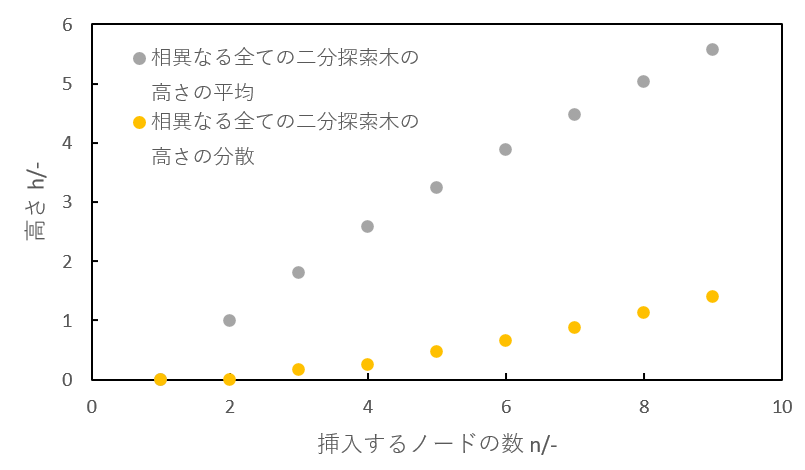
\includegraphics[width=6cm]{all_g.png}
\end{center}

\section{➂ 生成した二分探索木のうちAVL木または完全二分木の集合に対し、高さの平均・分散を算出}

AVL木および完全二分木の選別は以下の関数を用いて行った。

\begin{list}{\labelitemi}{\leftmargin=1em}
  \item count\_children : あるノードを根とした部分木の根を含むノード数を返す関数
  \item calculate\_hight : あるノードを根とした部分木の根の高さ+1の値を返す関数
  \item is\_AVL\_tree : あるノードを根とした部分木がAVL木であるかを判定する関数
  \item is\_complete\_binary\_tree : あるノードを根とした部分木が完全二分木であるかを判定する関数
\end{list}

is\_AVL\_tree関数は各ノードに対しcalculate\_hightを実行し左右の部分木の高さの差が1以内に収まっているかどうかを調べている。
同様にis\_complete\_binary\_tree関数は各ノードに対しcount\_childrenを実行し、左右の子ノード数の差が1以内に収まっているかどうかを調べている。

nが1から9までの場合についてそれぞれの木の高さの平均と分散を算出した。

\textrm{ACL木の場合}

\begin{center}
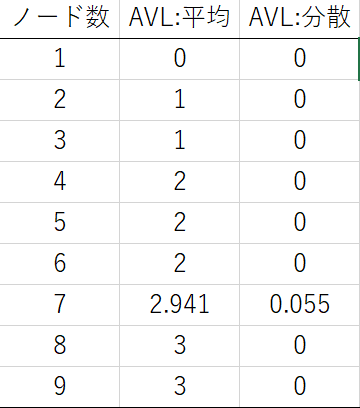
\includegraphics[width=5cm]{avl_t.png}
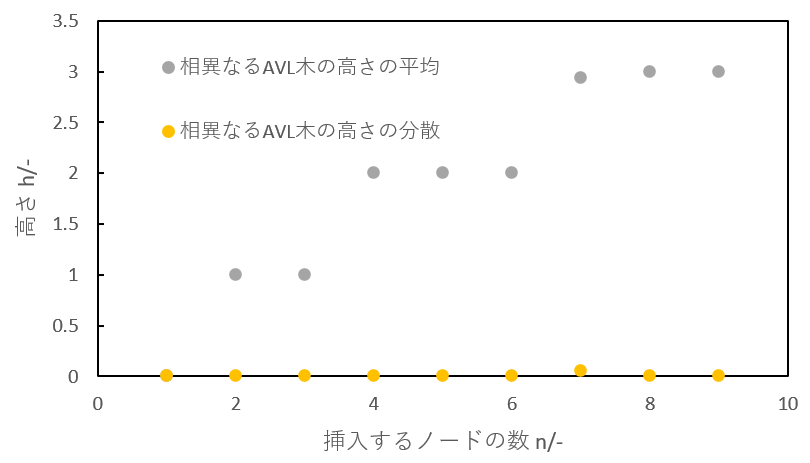
\includegraphics[width=6cm]{avl_g.png}
\end{center}

\textrm{完全二分木の場合}

\begin{center}
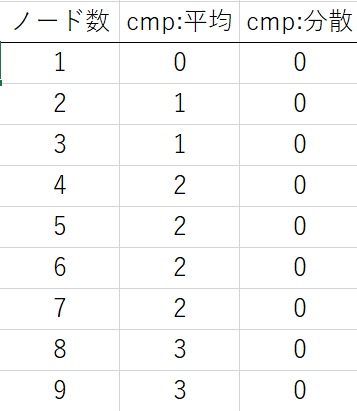
\includegraphics[width=5cm]{cmp_t.png}
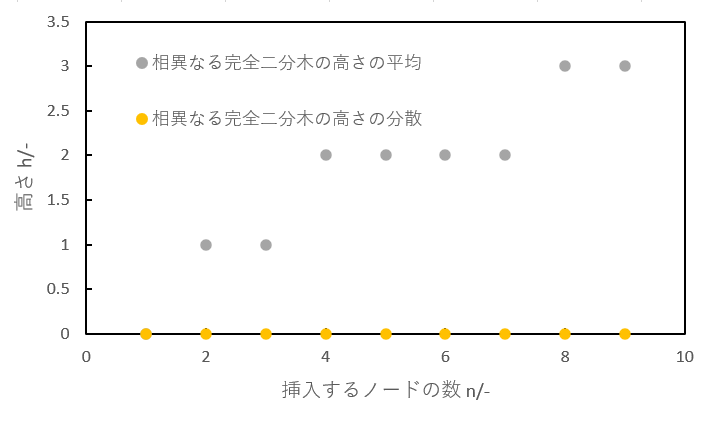
\includegraphics[width=6cm]{cmp_g.png}
\end{center}

➁と➂の結果をまとめそれぞれの高さの平均について比較したグラフをいかに示す。

\begin{center}
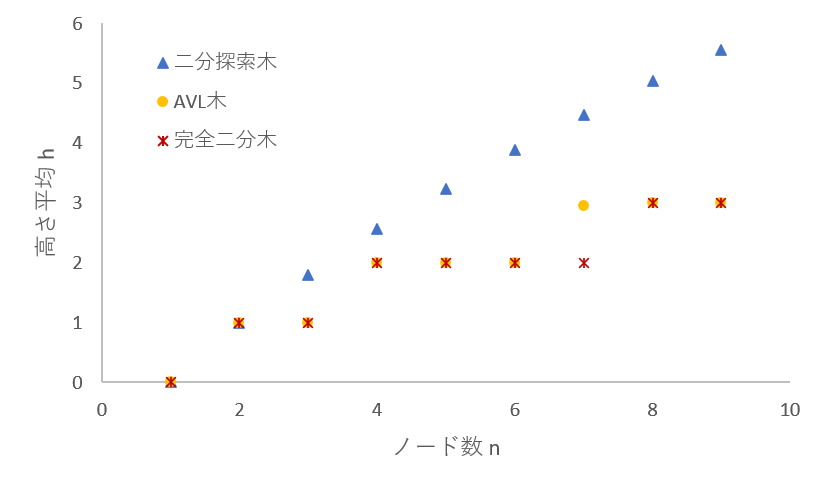
\includegraphics[width=8cm]{hikaku_g.png}
\end{center}

また、相異なる二分探索木の集合全体の要素数、AVL木のみの要素数、完全二分木のみの要素数を以下の図にまとめた。
なお、縦軸は対数軸である。

\begin{center}
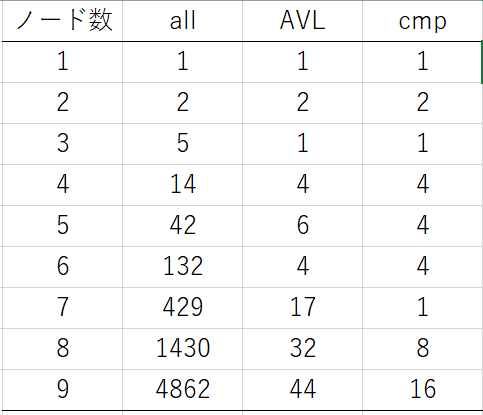
\includegraphics[width=5cm]{num_t.png}
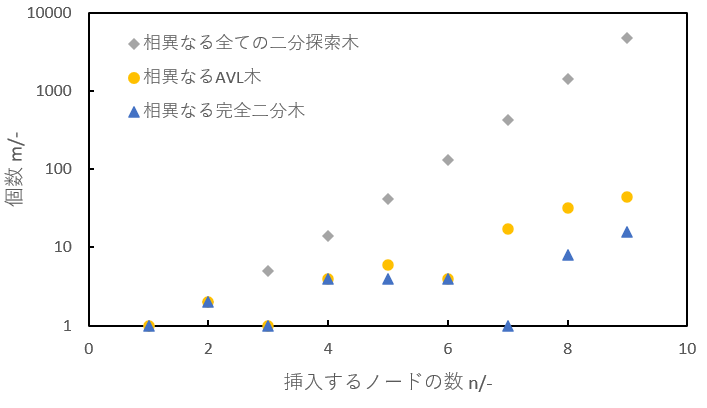
\includegraphics[width=6cm]{num_g.png}
\end{center}

\newpage

\section{ソースコード}

\subsection{ソースファイル}

\lstinputlisting[caption=binary_tree.c]{../binary_tree.c}

\lstinputlisting[caption=utility.c]{../utility.c}

\lstinputlisting[caption=tree_analysis.c]{../tree_analysis.c}

\lstinputlisting[caption=tree_graphic.c]{../tree_graphic.c}

\lstinputlisting[caption=simulation_graphic.c]{../simulation_graphic.c}

\lstinputlisting[caption=main.c]{../main.c}

\lstinputlisting[caption=list.c]{../list.c}

\lstinputlisting[caption=position.c]{../position.c}

\subsection{ヘッダファイル}

\lstinputlisting[caption=binary_tree.h]{../binary_tree.h}

\lstinputlisting[caption=utility.h]{../utility.h}

\lstinputlisting[caption=tree_analysis.h]{../tree_analysis.h}

\lstinputlisting[caption=tree_graphic.h]{../tree_graphic.h}

\lstinputlisting[caption=simulation_graphic.h]{../simulation_graphic.h}

\lstinputlisting[caption=list.h]{../list.h}

\lstinputlisting[caption=position.h]{../position.h}

最新のコードは以下のリンクから取得してください。

\url{https://github.com/zenon-paul/opengl_binary_tree}

\end{document}